\section{Local Filtering and Edge Detection}
\subsection{Filtering}
The naive approach of local filtering is taking just a moving average of the pixels in the neighbourhood.

\subsection{Convolution}
Convolve an input matrix (the input image) with a \textbf{kernel}, which is a matrix defining a weight for every element of the neighbourhood.
The convolution can be considered a moving weighted average of the pixels.
\begin{center}
	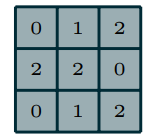
\includegraphics[width=0.4\linewidth]{img/Kernel_Convolution}
\end{center}
This kernel slides across the input matrix. At each location, the product between each element of the kernel and the input element it overlaps
is computed and the results are summed up to obtain the output in the current location.
In general, if the input matrix has  $i$ rows and the kernel has $k$ rows, the output will have $i-k+1$ rows, the same applies to columns.
\begin{center}
	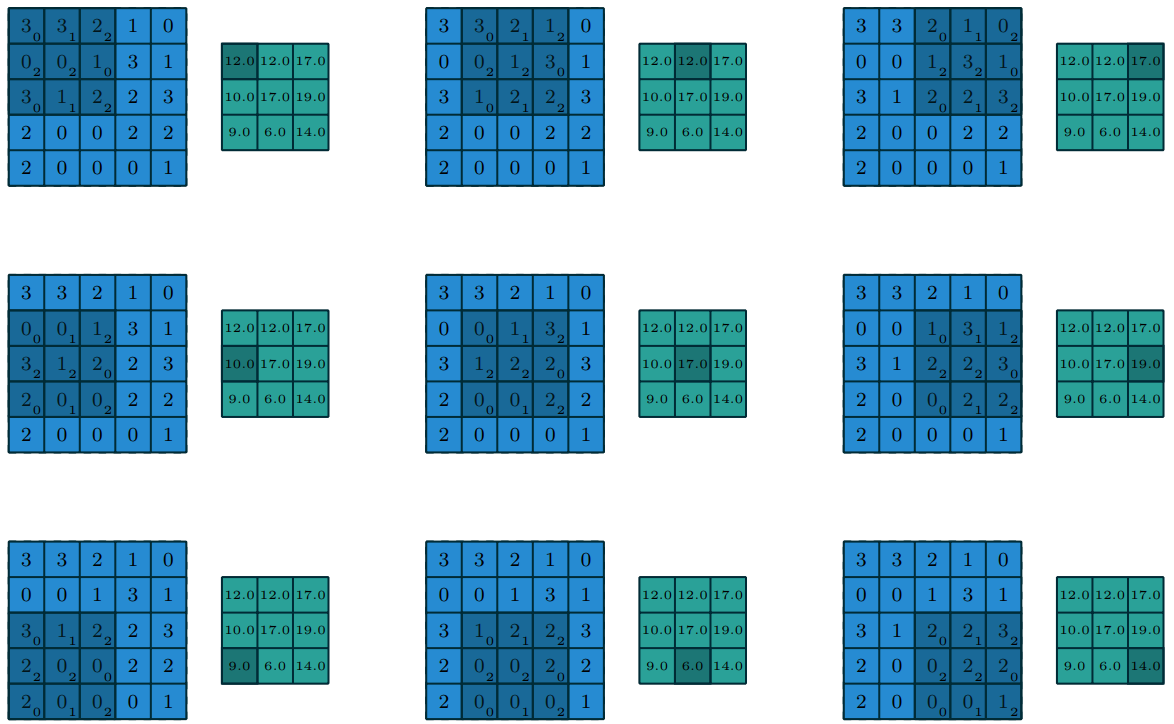
\includegraphics[width=0.8\linewidth]{img/ConvolutionOutput}
\end{center}

\subsection{Edge Detection}
Although intuitive for humans to detect, edge detection was a hard problem in image processing. An edge is defined by a rapid change in the intensity,
which can be exploited by calculating the derivative.

\begin{center}
	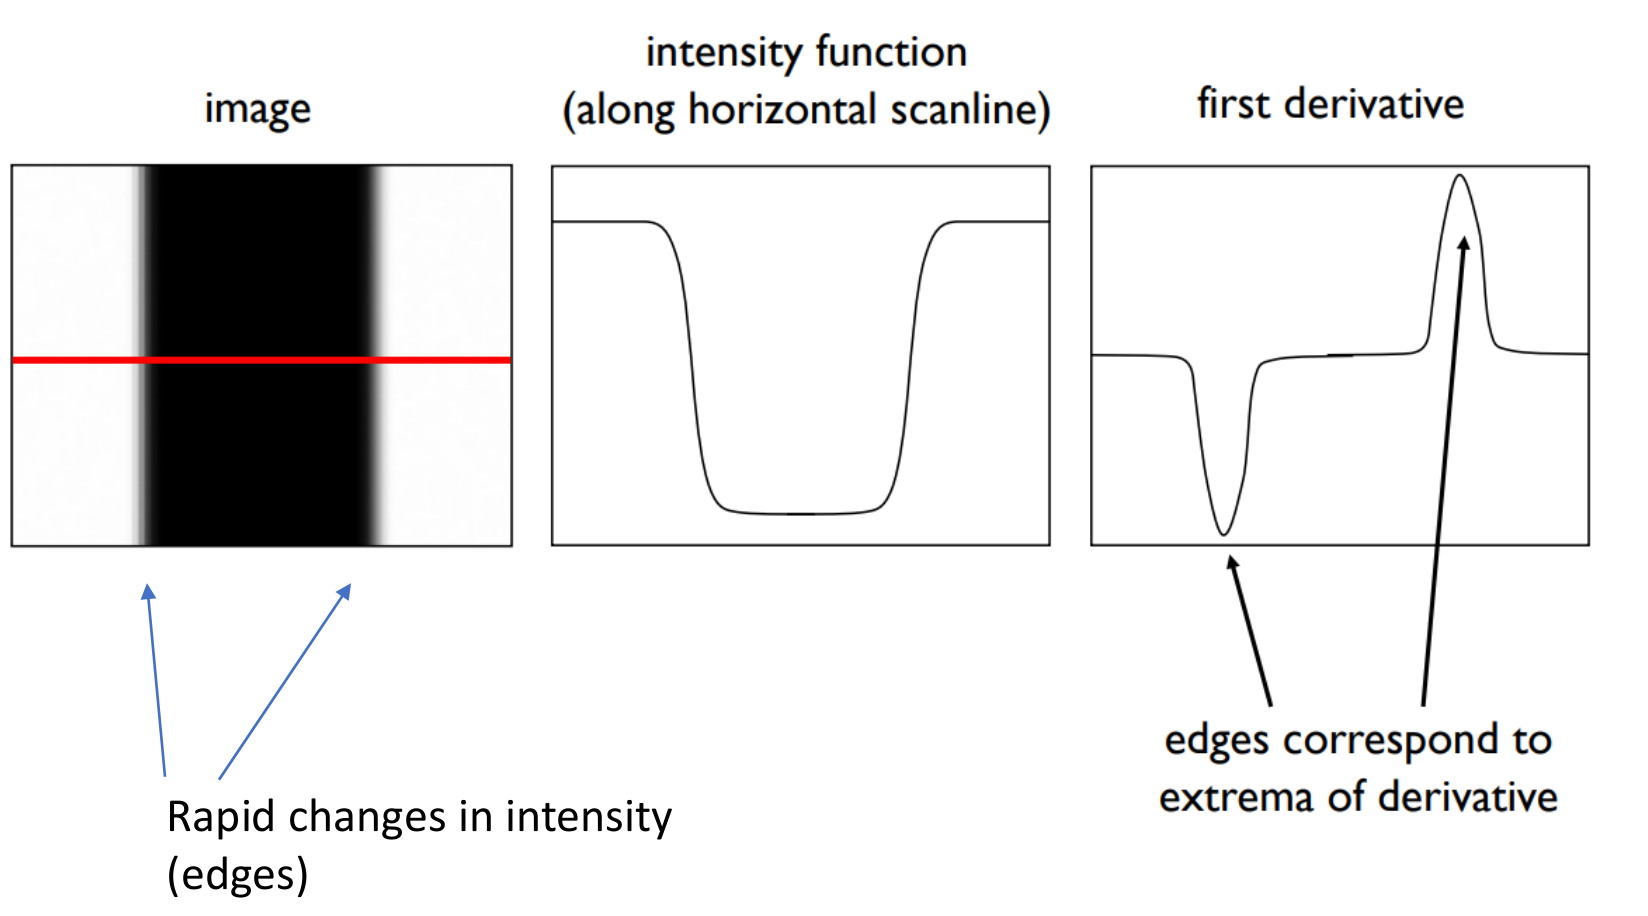
\includegraphics[width=0.6\linewidth]{img/1D_edge_derivative}
\end{center}

\noindent
In two dimensions the derivative corresponds to the gradient $\nabla f = \left[\frac{\partial f}{\partial x},\frac{\partial f}{\partial y}\right]$,
which points from the edge towards the increase in intensity or the lighter side.

\begin{align}
	& \text{Gradient} & \nabla f &= \left[ \frac{\partial f}{\partial x}, \frac{\partial f}{\partial y} \right] \\
	& \text{Gradient Direction} & \theta &= \tan^{-1} \left( \frac{\partial f}{\partial x} / \frac{\partial f}{\partial y} \right) \\
	& \text{Gradient Magnitude (or Modulus)} & \norm{\nabla f} &= \sqrt{\left(\frac{\partial f}{\partial x}\right)^2 + \left(\frac{\partial f}{\partial y} \right)^2 }
\end{align}

But not all important edges have strong gradients, nor are all strong gradients important edges.

\subsubsection{Computing the Gradient on an Image}
Approximate Gradient in direction of $ \frac{\partial f}{\partial x} $: Convolution with kernel \begin{tabular}{|c|c|}
	\hline
	-1 & 1\\
	\hline
\end{tabular}

\noindent
Approximate Gradient in direction of $ \frac{\partial f}{\partial y} $: Convolution with kernel \begin{tabular}{|c|}
	\hline
	-1 \\
	\hline
	1\\
	\hline
\end{tabular}

The drawback of the gradient is, that it is very sensitive to noise:
\begin{figure}[H]
	\centering
	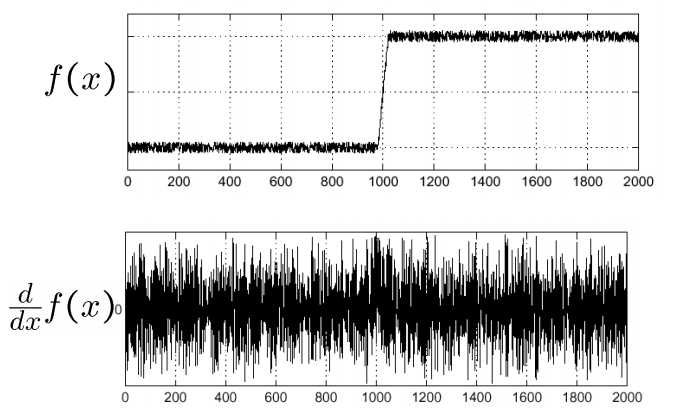
\includegraphics[width=0.7\linewidth]{noise_gradient}
	\caption{Gradient of a 1D function, where it is clear how it amplifies noise and may conceal a weak signal}
	\label{fig:noisegradient}
\end{figure}

\noindent
The solution to this is, to first smooth the function and then apply the gradient.

The larger the value of $\sigma$ the more smoothing is applied and different kind of features can be identified.
\begin{itemize}[leftmargin=*, labelindent=3.5cm, labelsep=0.5cm]
	\item[\textbf{large value of $\sigma$}] larger scale or stronger edges detected
	\item[\textbf{smaller value of $\sigma$}] finer details detected
\end{itemize}

\noindent
\begin{minipage}{0.6\textwidth}
	In practice a convolution with a derivative of Gaussian filter is calculated to compute the gradients.

	This is equivalent to smoothing with a Gaussian and then taking the derivative.
\end{minipage}
\begin{minipage}{0.4\textwidth}
	\begin{center}
		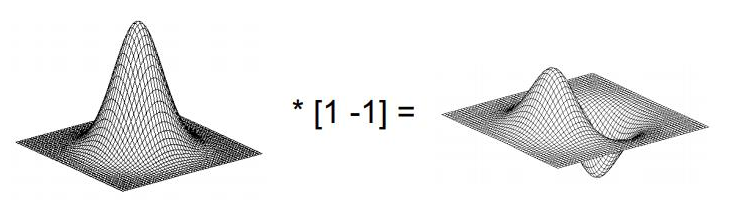
\includegraphics[width=0.6\linewidth]{img/derivative_gaussian_filter}
	\end{center}
\end{minipage}

\begin{figure}[H]
	\centering
	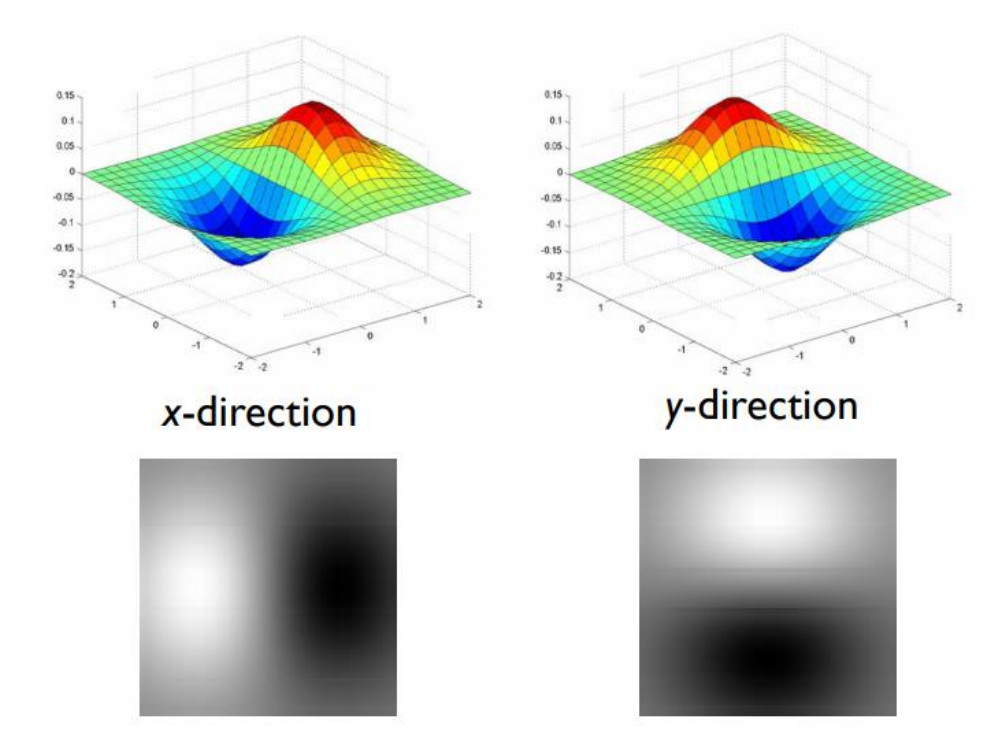
\includegraphics[width=0.6\linewidth]{img/derivative_gaussian_filter2}
	\caption{Derivative of Gaussian Filters}
	\label{fig:derivativegaussianfilter2}
\end{figure}

\begin{itemize}
	\item A Gaussian smoothing filter removes high-frequency components
	\item Values of a Gaussian smoothing filter sum to one
	\item Derivative filters contain some negative value and values sum to zero
	\item Derivative filters yield large responses at points with high contrast
\end{itemize}

\subsection{Canny Edge Detection}
Same base approach but enhanced with edge thinning and hysteresis thresholding.\footnote{A good explanation with sample code can be
found under \href{https://docs.opencv.org/4.3.0/da/d22/tutorial_py_canny.html}{OpenCV Canny Edge Detection Tutorial}}
\begin{enumerate}
	\item Approximate gradients along axes by derivative of Gaussian filters
	\item Compute gradient magnitude
	\item Make edge one pixel wide, thinning through \textbf{non-maxima suppression} along perpendicular direction to the edge
	\item Only keep strong edges through hysteresis thresholding
\end{enumerate}

\subsection{Hysteresis Thresholding}

\begin{wrapfigure}{R}{0.4\textwidth}
	\centering
	\vspace{-16mm}
	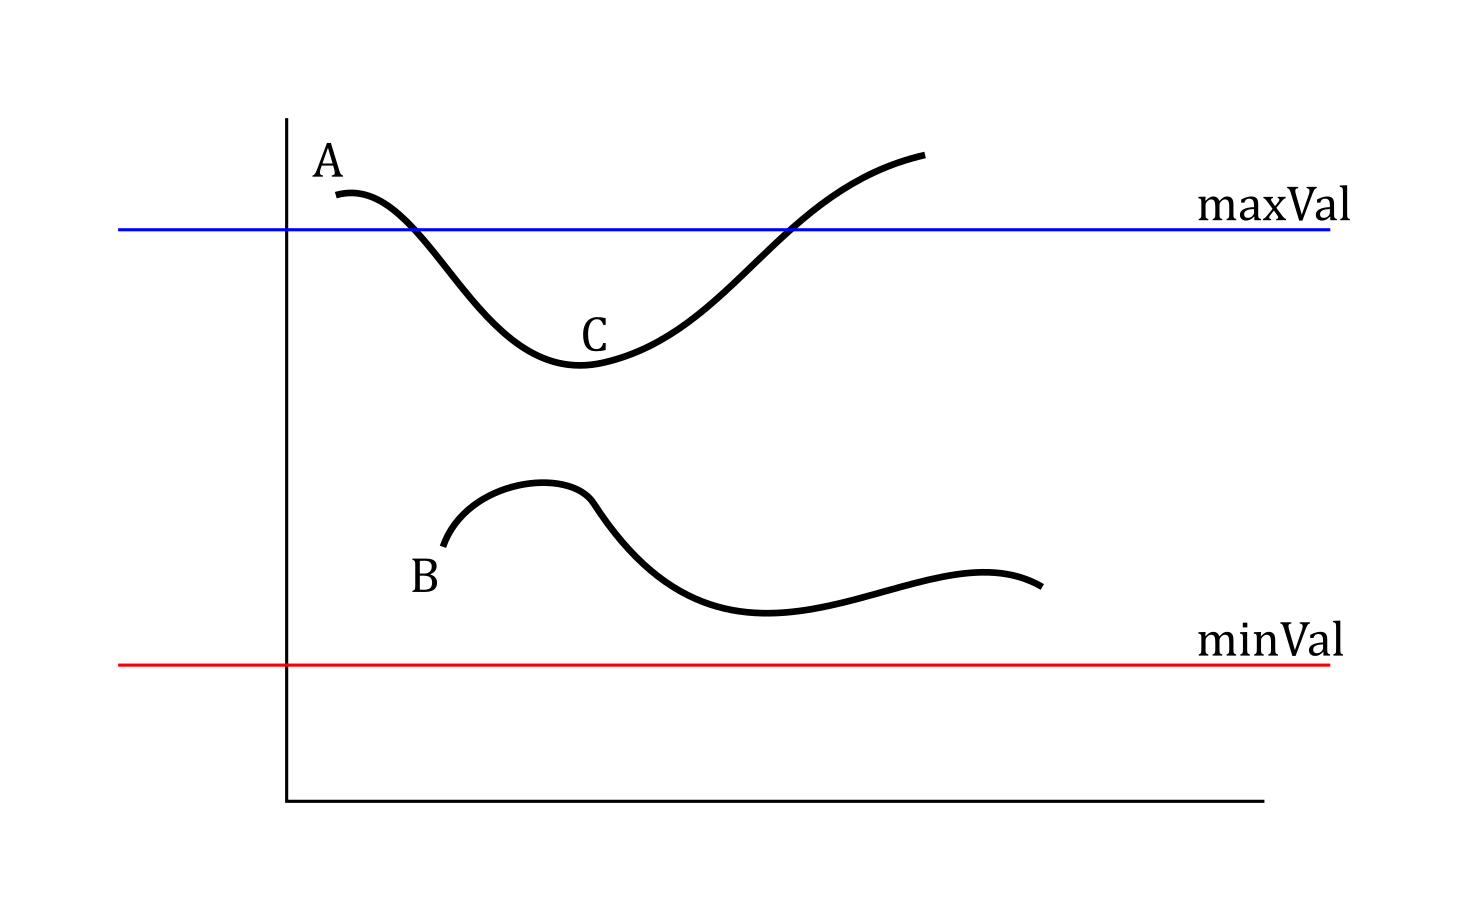
\includegraphics[width=\linewidth]{hysteresis_thresholding}
	\vspace{-20mm}
\end{wrapfigure}

This stage determines genuine edges by employing two threshold values, minVal and maxVal.
Edges with an intensity gradient surpassing maxVal (A) are definitively identified as edges,
while those falling below minVal are discarded as non-edges.
Pixels lying between these thresholds are classified based on connectivity:
if connected to ``sure-edge'' pixels (C), they are deemed part of edges; otherwise (B), they are also discarded.

% \begin{figure}[H]
% 	\centering
% 	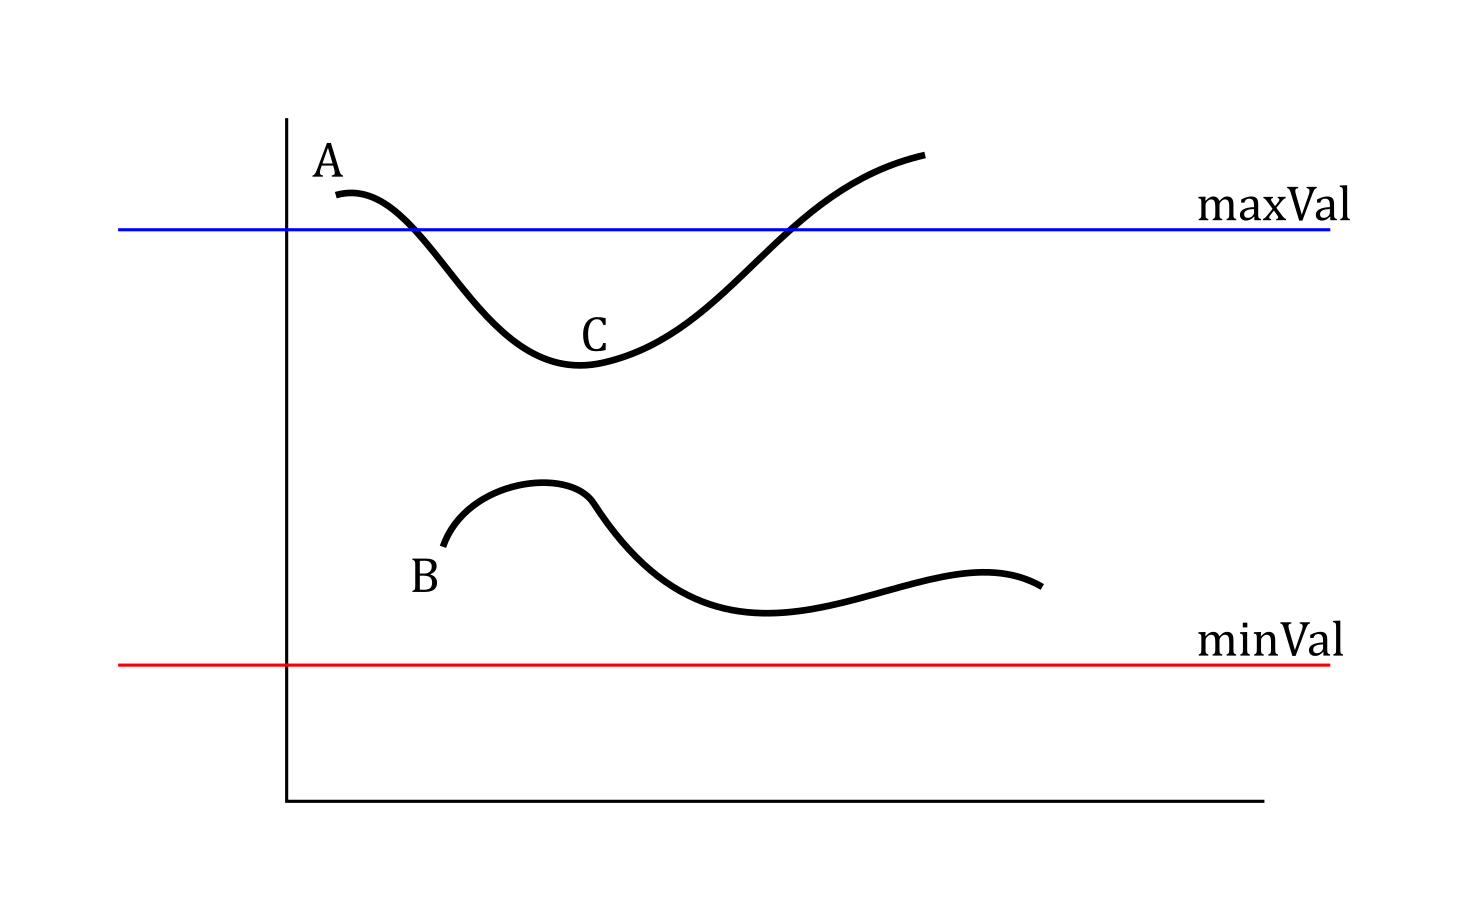
\includegraphics[keepaspectratio,width=0.6\linewidth]{hysteresis_thresholding}
% 	\caption{Hysteresis thresholding with A) sure edge, B) non-edge and C) a non-edge connected to a sure edge}
% \end{figure}
